% !TeX program = xelatex
\documentclass[a4paper]{scrarticle}

\usepackage[ngerman]{babel}
\usepackage[utf8]{inputenc}
\usepackage[T1]{fontenc}

\usepackage[left=2.25cm, right=2.25cm, top=3.00cm, bottom=3.50cm]{geometry}
\usepackage[headsepline, footsepline]{scrlayer-scrpage}
\renewcommand*{\headfont}{\normalfont}
\usepackage{csquotes}

\usepackage{graphicx}
\graphicspath{ {./images/} }
\usepackage[figurename=Abb.]{caption}
\usepackage{floatrow}

\usepackage{amsmath}
\usepackage{amssymb}

\usepackage{tabto}
\usepackage{xcolor}
\usepackage{enumitem}
% \usepackage{blindtext, showframe}
\usepackage{fontspec}

\usepackage{pdfpages}


\definecolor{AKSAcolor}{rgb}{0.9,0.0,0.0}
\newfontfamily\AKAfont{AKA}

% Redefine sectioning commands to set font
\makeatletter
\renewcommand\section{\@startsection {section}{1}{\z@}%
                                   {-3.5ex \@plus -1ex \@minus -.2ex}%
                                   {2.3ex \@plus.2ex}%
                                   {\Huge\AKAfont}}
\renewcommand\subsection{\@startsection{subsection}{2}{\z@}%
                                     {-3.25ex\@plus -1ex \@minus -.2ex}%
                                     {1.5ex \@plus .2ex}%
                                     {\Large\AKAfont}}
\renewcommand{\maketitle}{%
																		 \begin{titlepage}
																			 \null\vfill % Add space at the top
																			 \begin{center}
																				{\huge\@title\par}%
																				\vspace{0.5cm} % Adjust spacing between title and author
																				{\large\@subtitle\par} % Add the subtitle
																				\vspace{1.5cm} % Adjust spacing between author and subtitle
																				{\Large\@author\par}
																				\vspace{2.5cm} % Adjust spacing between subtitle and date
																				\begin{center}
																					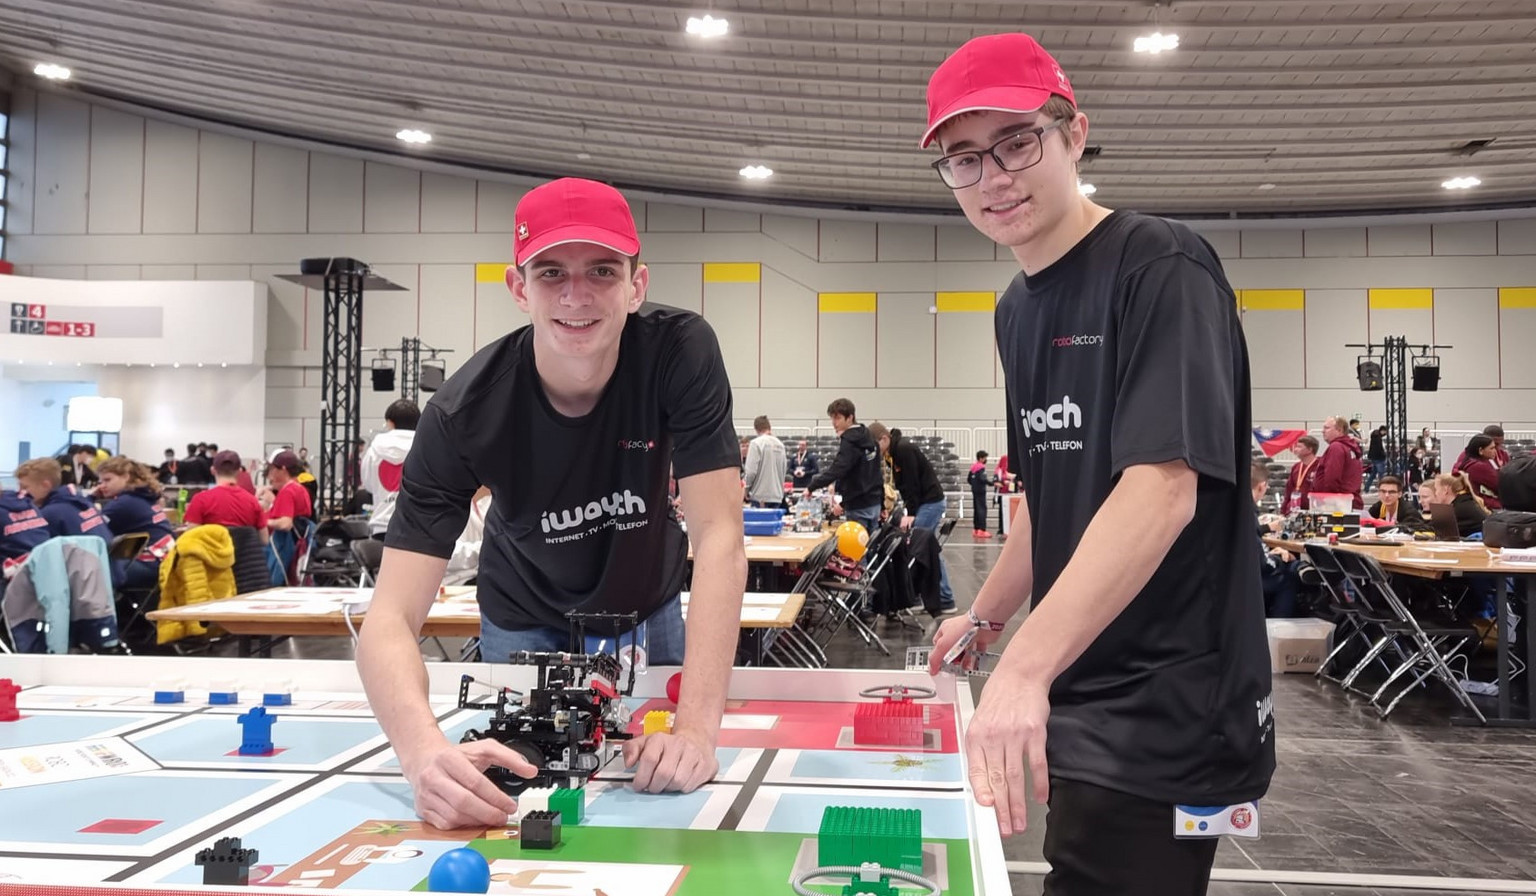
\includegraphics[width=15cm]{team}
																				\end{center}
																				\vfill
																				\vspace{0.5cm} % Adjust spacing between subtitle and date
																				{\large\@date\par} % Add the date
																				Eingereicht bei der WRO Regio in Waldkirch bei Freiburg
																			 \end{center}
																			 \@thanks % If you have any thanks or notes, they will be printed here
																		 \end{titlepage}%
																	 }

\makeatother

\usepackage{hyperref}
\hypersetup{colorlinks=false, pdfborder={0 0 0}, pdftitle=}



\begin{document}

\title{\AKAfont\Huge\textcolor{AKSAcolor}{Dokumentation}}
\subtitle{Future Engineers 2024}
\author{robofactory (Jesse Born, Julian von Hoff)}
\date{April 2024}

\pagenumbering{gobble} % Suppress page numbering
\ihead{Future Engineers Dokumentation}
\ifoot{\\robofactory, 2024}

\maketitle
\clearpage
\newpage


\pagenumbering{arabic}

\section{Motorisierung}

Als Hauptantrieb verwenden wir eine Handelsübliche Kombination aus Fahrtenregler und Motor, die aus dem Modellbau stammt.
Wir nutzen wir einen 21.5 T gewickelten BLDC/brushless Motor von Tamiya mit eingebautem Drehgeber und das dazugehörige ESC TBLE-04SR. 
Über ein Differenzialgetriebe und eine gesamthafte Untersetzung um den Faktor 3.122:1 bringt unser Fahrzeug seine Motorleistung über einen Heckantrieb auf den Boden.
Unsere Räder bestehen aus Felgen, die im Lieferumfang unseres Chassis dabei waren, so wie 56x28 mm Reifen von LEGO.

Zur Steuerung des Roboterautos ist ein "Amewi AMX Racing DC5821LV" Servo verbaut. Dieser wurde aufgrund der hohen Auflösung und Geschwindigkeit gewählt.

Um mit dem Raspberry Pi das ESC und den Servo anzusteuern, werden 2 PWM-Ausgänge benötigt. Mit einem eigenen HAT, der direkt auf den 40-Pin-Erweiterungsstecker des Pi gesteckt werden kann, brechen wir diese Stecker passend aus.
\section{Energie \& Sensoren}

Der einzige Sensor, den wir verbaut haben, ist eine RGB-D Kamera von Orbbec, eine "Astra Embedded S".
Dieses verhältnismässig preiswerte Auslaufprodukt ermöglicht nebst der klassischen Webcamfunktion auch das Erfassen von Tiefeninformation mithilfe von strukturiertem Infrarotlicht.
Via USB / UVC-Protokoll wird das Kamerabild an unseren Hauptrechner, einen Raspberry Pi 4B übertragen.


Die Stromversorgung erfolgt über einen sechszelligen NiMh-Akku. Um den Raspberry Pi mit Strom zu versorgen, wird ein BEC (Battery Eliminator Circuit) aus dem Modellbau verwendet. 
Mit den Pins 2 und 6 des GPIO-Headers des Pi wird dieser schlussendlich mit Strom versorgt.
Genau dieses technische Detail bereitete uns am meisten Kopfschmerzen sowie ein totes Raspberry Pi. Wir konnten jedoch nicht genau feststellen, weshalb der Pi seinen "magischen Rauch" freigab. Unsere beste Hypothese ist eine fehlende "flyback" Diode.

\section{Hindernisse \& Algorithmen}

Das von unserer Kamera erfasst RGB- bzw. BGR-Bild folgt nun 2 Pfaden: Der erste ist dafür zuständig, während dem Hindernisrennen die farbigen Hindernisse zu registrieren. Entlang dem zweiten Pfad werden mittels Graustufenbild und Hough-Lines-Algorithmus die Banden des Spielfeldes erfasst und auf einem virtuellen Spielfeld lokalisiert.

\subsection{Banden}

Als erstes erstellen wir ein Bild, in dem nur alle (fast) schwarzen Pixel abgebildet sind. Darin suchen wir anschliessend nach kontrastreichen Kanten.
Haben wir die Kanten gefunden, segmentieren wir mittels probabilistischer Hough-Transformation zusammenhängende Kanten aus.
Nun filtern wir diese Ecken weiter, wir überspringen dabei alle Linien, welche:
\begin{enumerate}
	\item {keinen Endpunkt in einem 80 Pixel hohen Streifen um die Bildmitte haben}
	\item {eine Länge von Null haben}
	\item {komplett über der Bildmitte liegen}
	\item {vertikal im Bild stehen}
\end{enumerate}
So erhalten wir pro Wand eine Linie an der unteren Kante dieser an der Stelle, wo sie auf die Spielfeld-Matte trifft.
Mittels des 2. Strahlensatzes können wir nun den Abstand schätzen.
$$
d = \frac{1}{(y_{Endpunkt}-y_{Bildmitte})} * s_d
$$
($d$: Abstand, $y_{Endpunkt}$: y-Koordinate eines Linienendpunktes im Bild, $y_{Bildmitte}$: Parallaxenmitte des Kamerbildes und $s_d$: konstanter Faktor, der sich zwar aus den intrinsischen Kameraparametern ableitet, jedoch experimentell bestummen wurde. )

Wände werden nun in drei Klassen unterteilt:
\begin{itemize}
	\item Rechts: Eine Wand am rechten Bildrand
	\item Links: Eine Wand am linken Bildrand
	\item Mitte: Eine Wand, deren Steigungswinkel unter $0.05$ (rad) liegt.
\end{itemize}
Diese Klassifizierung wird auch zu Beginn des Laufs zur feststellung der Rundenrichtung verwendet – ist eine linke Wand sichtbar, wird im Uhrzeigersinn gefahren.


\subsection{Startrichtung}

Zu Beginn des Laufs ist nur jeweils eine mittlere Wand sowie eine rechte oder linke Wand sichtbar.
Ist eine linke Wand sichtbar, ist die Umlaufrichtung für diese Runde im Uhrzeigersinn – ist es eine rechte Wand im Gegenuhrzeigersinn.

\subsection{Farbene Hindernisse}

Das originale RGB-Bild wird in den HSV-Farbraum umgerechnet, um rot und grün deutlich unterscheiden zu können. Diesen Trick kennen und nutzten wir bereits seit mehreren Jahren in der Kategorie RoboMission der WRO.
Pixel, die jetzt zwischen der Rot- oder Grüngrenzen liegen, werden als der Farbe entsprechend gespeichert. 
Auf diesen Binärbildern werden nun die Konturen erkannt und die Mittelpunkte sowie die Breite und Höhe bestummen.

Analog zu oben, jedoch nur mit der Höhe des erkannten Umrisses, wird mittels Strahlensatz der Abstand zum Hindernis geschätzt.

\subsection{Steuersignal}

Mit dem Abstand gewichtet, wird nun für jedes erkannte Objekt, also Banden und Hindernisse, dessen bevorzugte Richtung in einen Wert summiert.
\[
	s := \frac{\sum_{}\frac{1}{d_i}}{T}
\]
Dieser Wert wird dann auf das geschlossene intervall $[-1;1]$ normalisiert. Der normalisierte Wert wird dann auf den Lenkanschlag des Servos abgebildet, so dass 0 auch einem gerade getrimmten Auto entspricht.
\[
	\alpha := [\frac{s}{16.0}]_{-1}^{ 1}	
\]
		
\subsection{Ende der Runde}

Um am Ende der Runde im Startbereich stoppen zu können, zählen wir, wie oft wir um eine Ecke biegen.
Mittels Auswerten der an den Roboter ausgegebenen Steuersignale wird eine Ecke identifiziert und eine Variable wird um eins erhöht.
Sobald diese Variable 12 erreicht wird der Lauf im nächsten geraden Bereich gestoppt. 
\subsection{Programmierung}

Bei der Programmierung setzen wir auf Python. Wir setzten ausserdem extensiv auf die Pakete opencv-python sowie NumPy.
Mittels dieser Pakete erreichen wir einen hohen Grad an paralleler Bildverarbeitung, was uns eine Verarbeitungsrate von ca. 30 Hz ermöglicht (wenn die Kamerabilder nicht per WiFi gestreamt werden).

Der Code wird bewusst funktional gehalten, nur vereinzelt werden objektorientierte Muster genutzt.
\begin{figure}[ht]
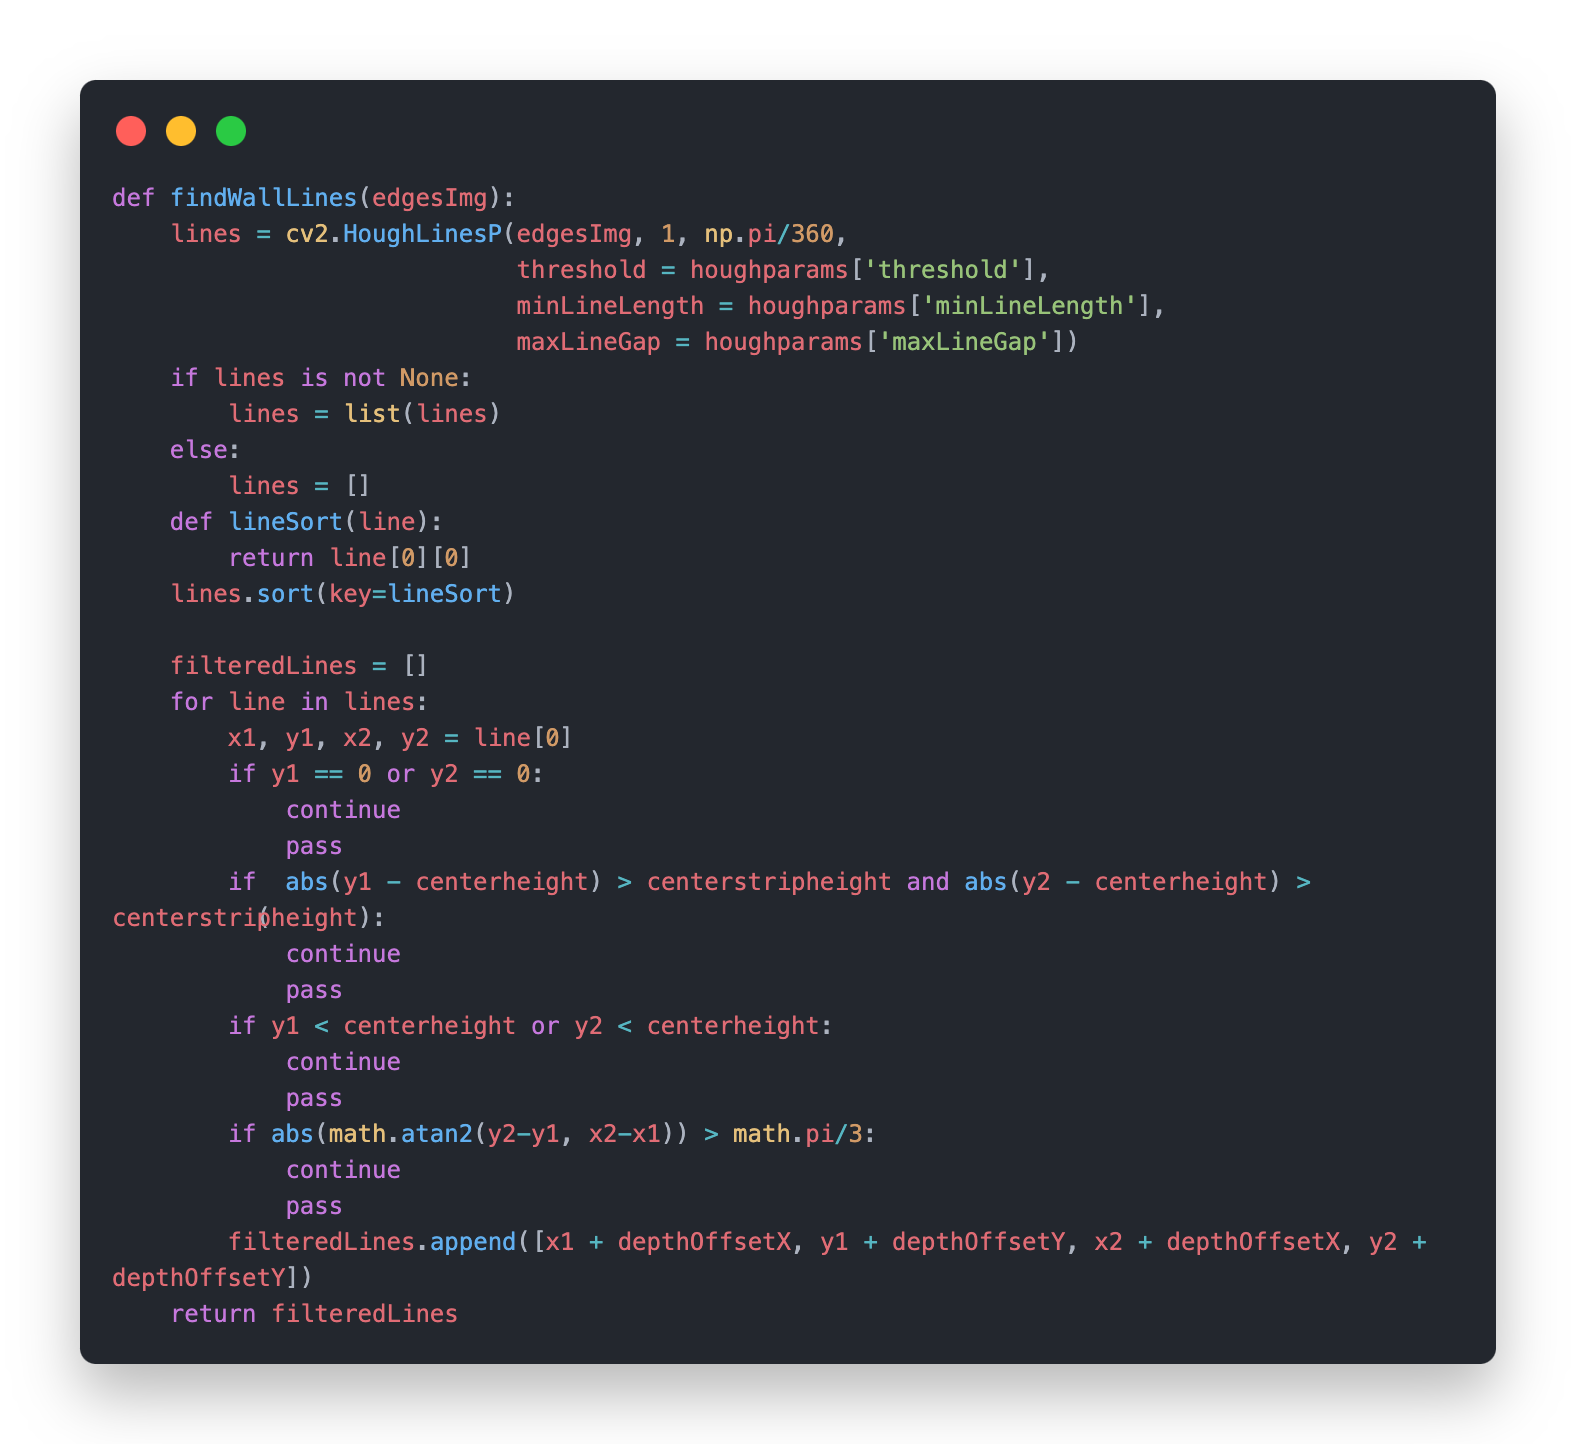
\includegraphics[width=15cm]{findWallLines.png}
\caption{Auszug aus dem Code: Wanderkennung}
\end{figure}
\begin{figure}[ht]
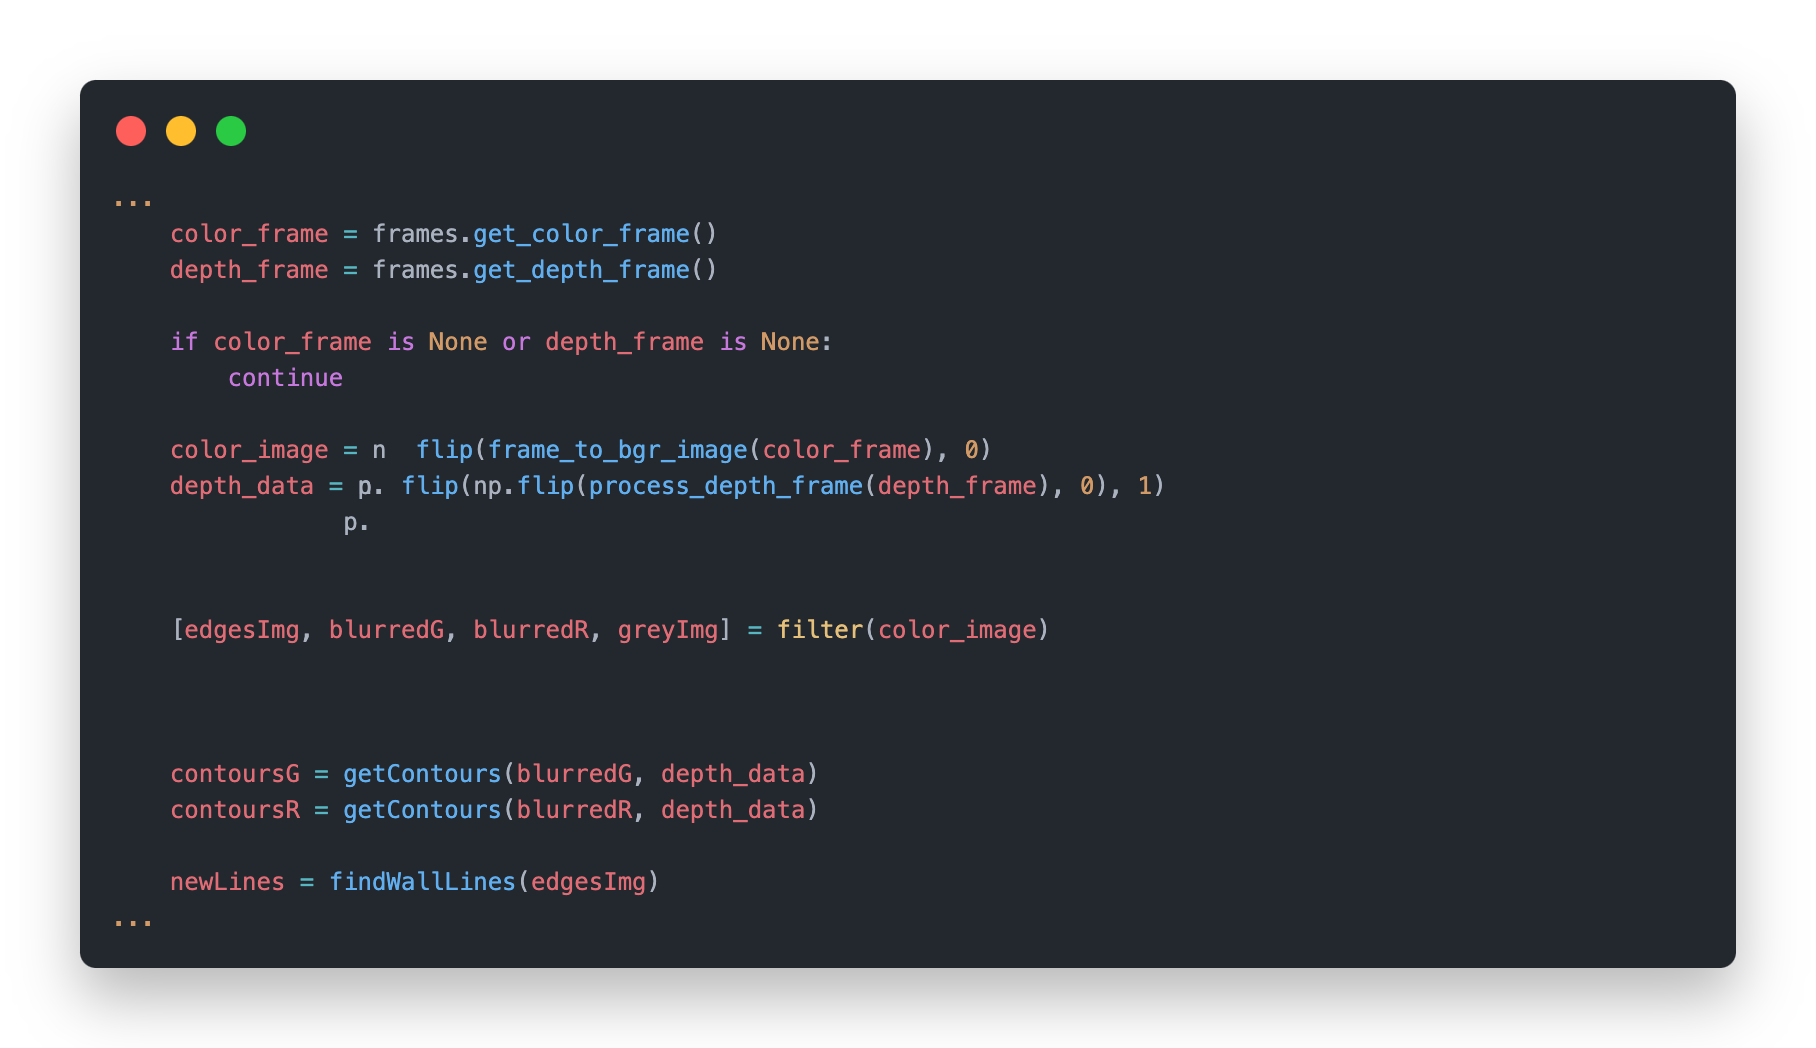
\includegraphics[width=15cm]{mainloop.png}
\caption{Auszug aus dem Code: Hauptschleife}
\end{figure}
\begin{figure}[ht]
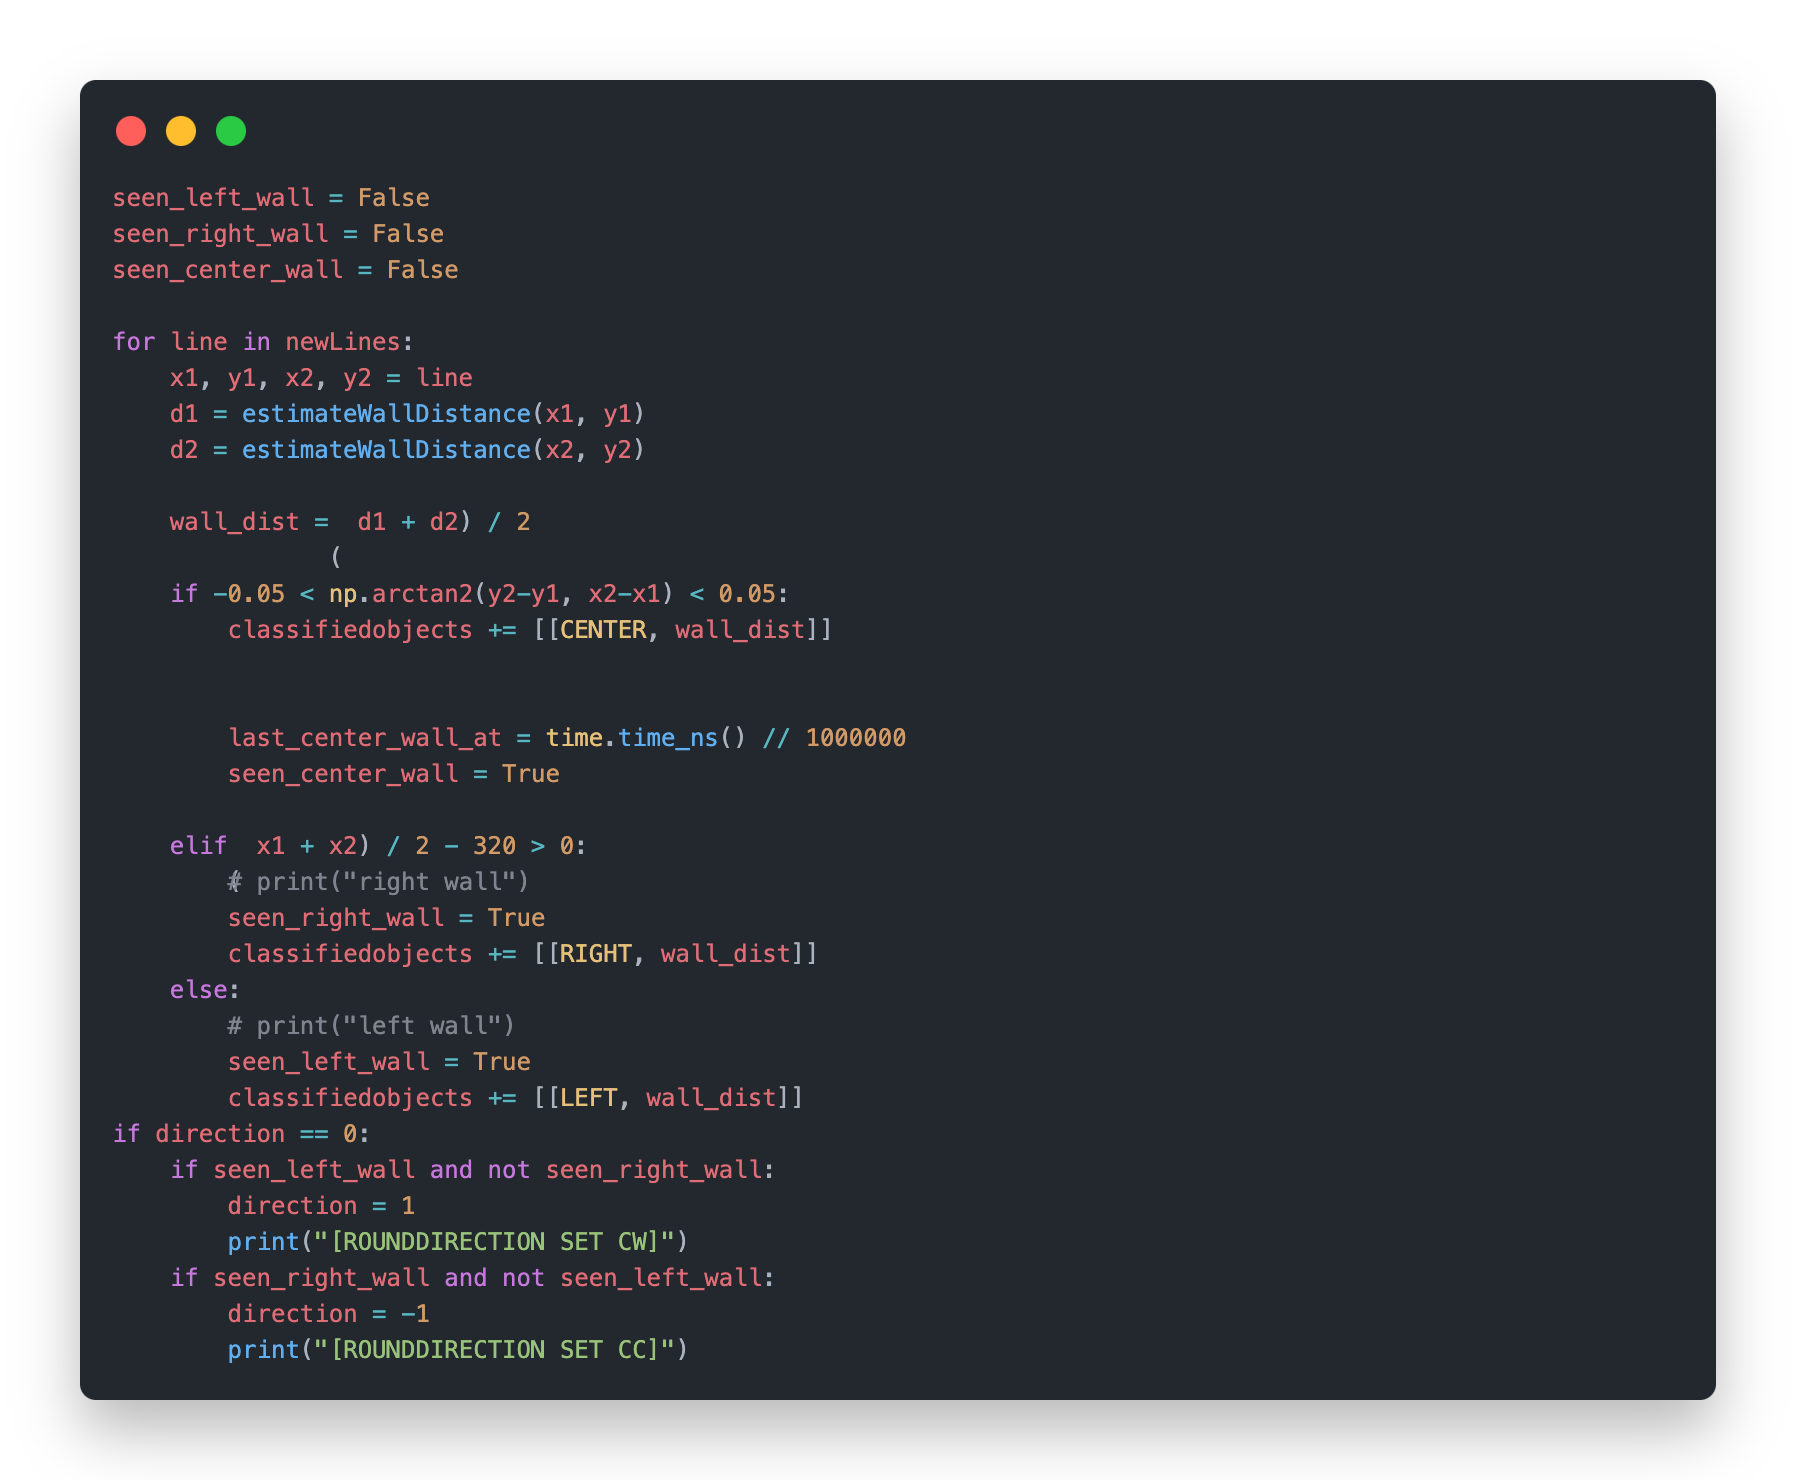
\includegraphics[width=15cm]{classification.png}
\caption{Auszug aus dem Code: Wandklassifizierung}
\end{figure}


\clearpage
\section{Fotos}
\begin{center}
	\includegraphics[width=14cm]{iso.png} \\		
	\includegraphics[width=14cm]{labeled.png} \\		
	\begin{tabular}{ c c }
		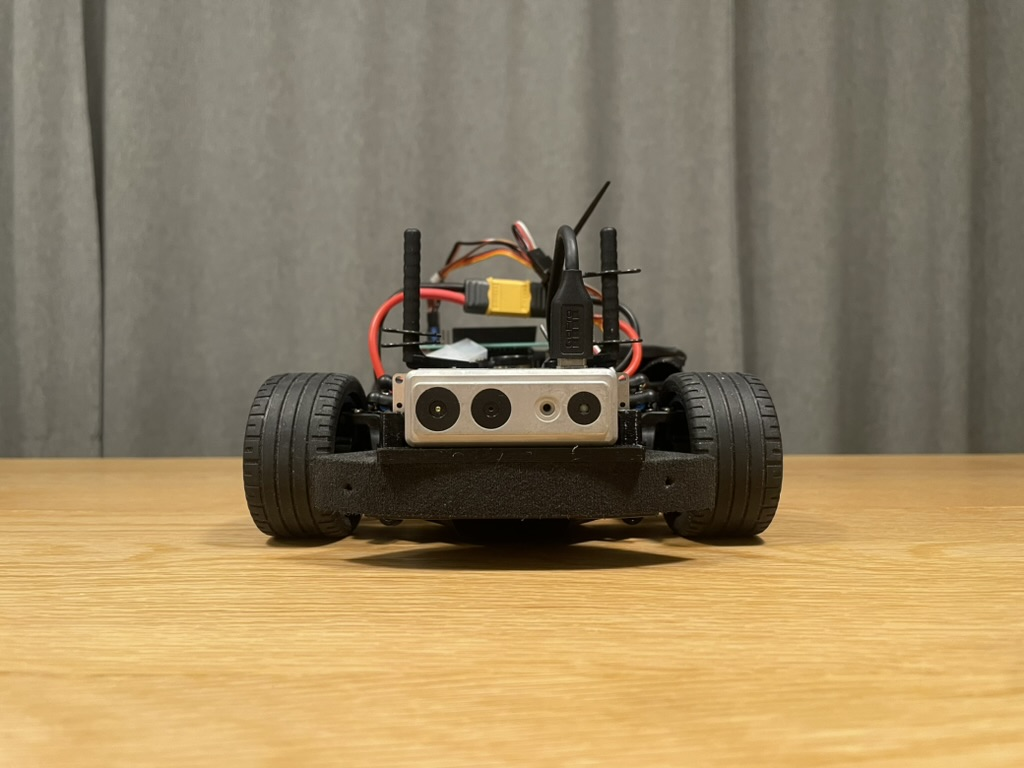
\includegraphics[width=7cm]{front.jpeg} & 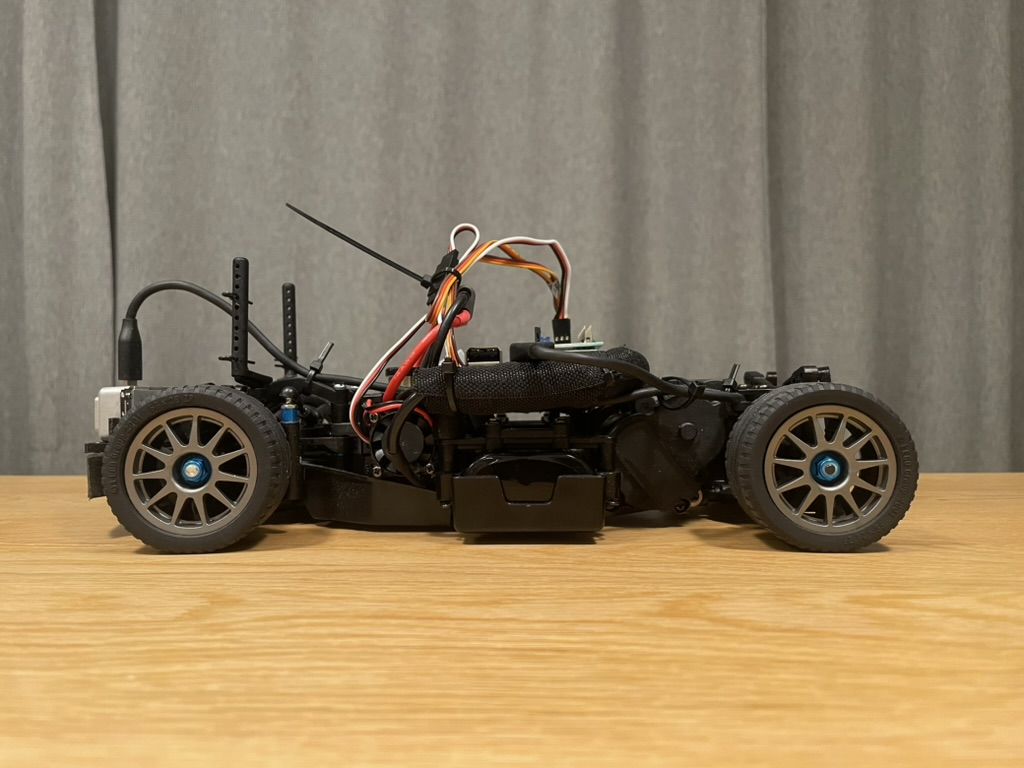
\includegraphics[width=7cm]{left.jpeg} \\ 
		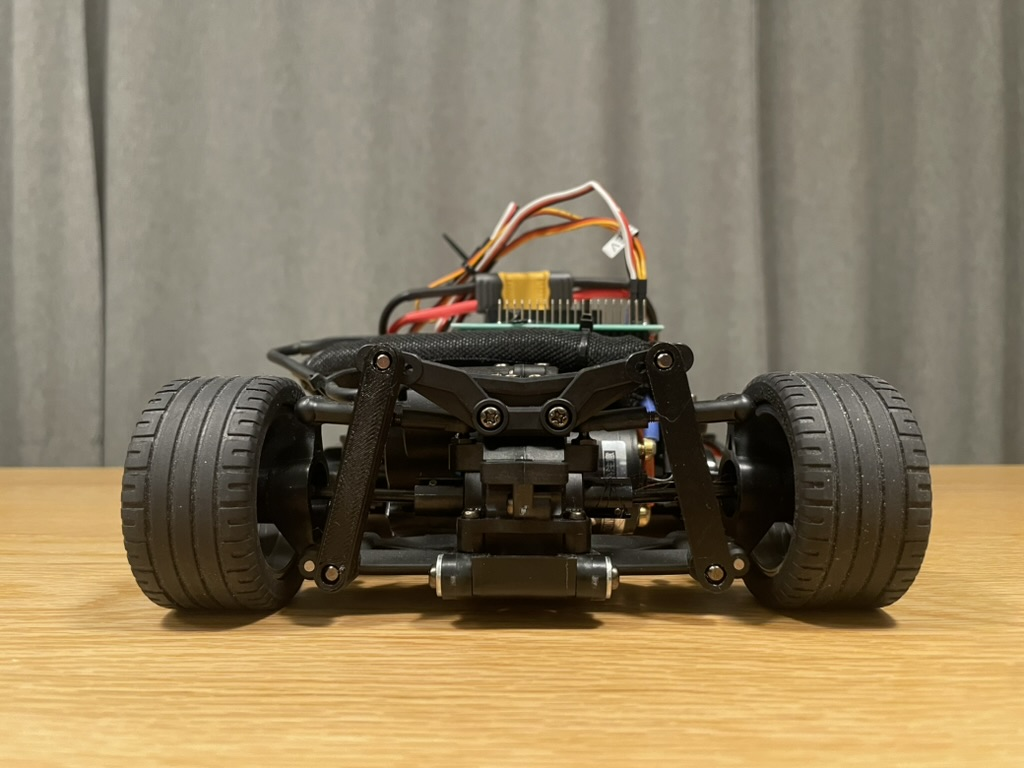
\includegraphics[width=7cm]{rear.jpeg} & 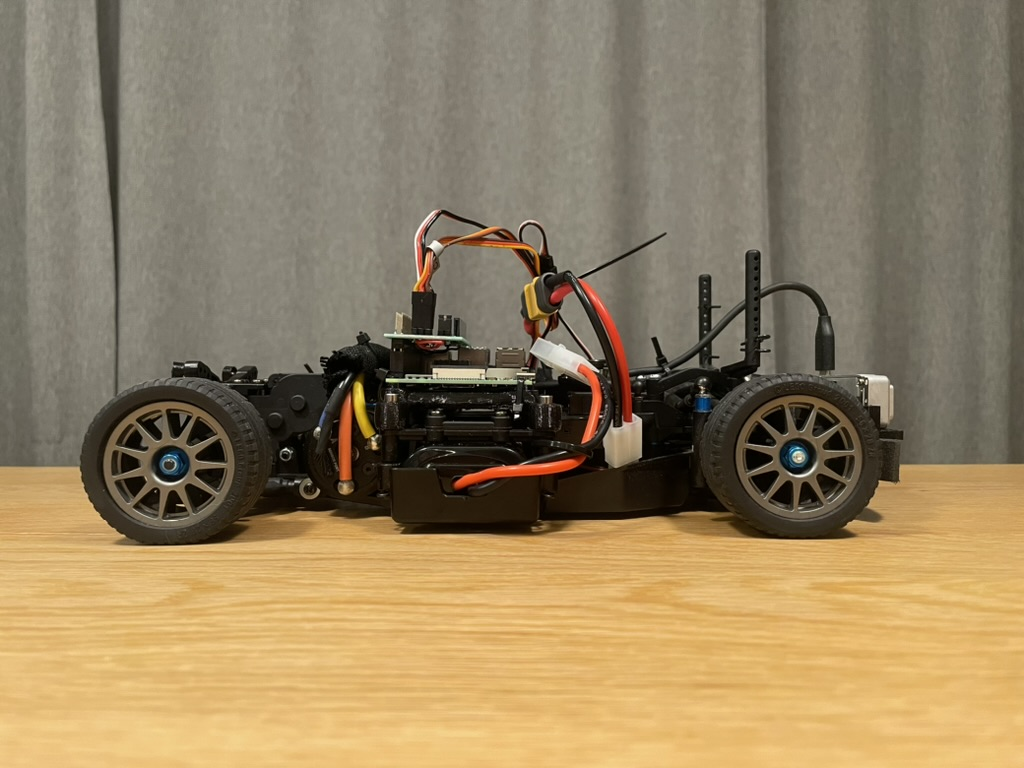
\includegraphics[width=7cm]{right.jpeg} \\  
		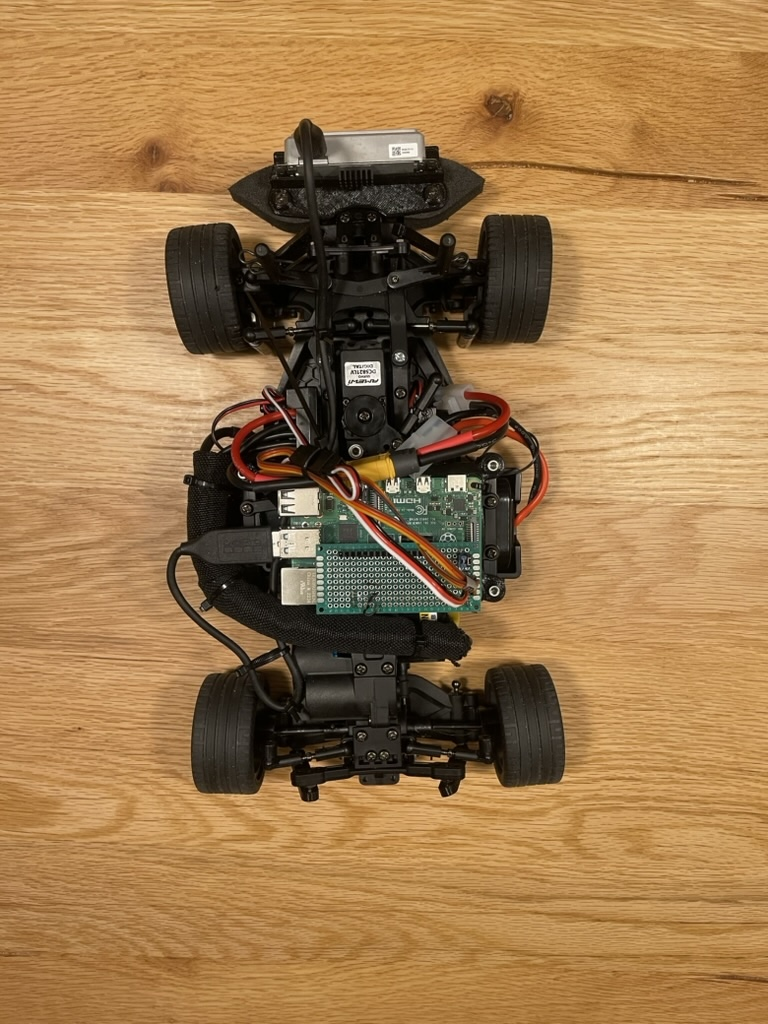
\includegraphics[width=7cm]{top.jpeg} & 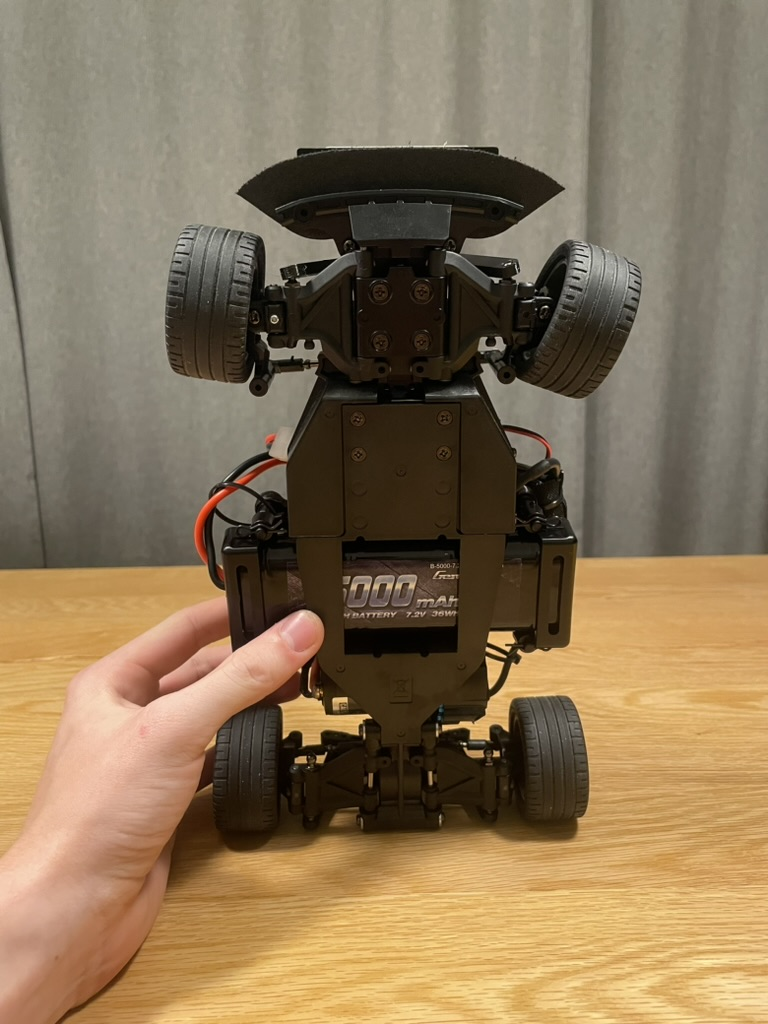
\includegraphics[width=7cm]{bottom.jpeg}    
	\end{tabular}
\end{center}
\clearpage

\section{Engineering \& Design}
Der Bausatz des Chassis stammt ebenfalls aus dem Hause Tamiya – den Klassiker M-08 Concept haben wir modifiziert, dass der Einschlag der Lenkung grösser und die Federung so steif wie nur möglich ist. (Siehe Kapitel "3 - Hindernisse").
Die vordere Stossstange, bestehend aus einem dichten Schaumstoff haben wir an der Bandsäge gekürzt, sodass die Gesamtlänge des Autos auch in die vorgegebenen 300 mm passt.
Ergänzt haben wir den fahrbaren Unterbau mit einer Kamerahalterung über der vorderen Stossstange. Die Kamera hält darin reibungsbasiert und lässt sich für Wartungsarbeiten rund um diese leicht entfernen.
Aus Notdurft – um unseren Wanderkennungsalgorithmus zu unterstützen – haben wir die hydraulische Federung des Chassisbausatzes mit soliden, 3-D-gedruckten Teilen ersetzt. Damit vermeiden wir, dass unser Auto rollt oder nickt – denn dies macht die visuelle Distanzschätzung ungenau bis unbrauchbar.
Um unsere Recheneinheit auf dem Auto zu befestigen, haben wir eine Halterung 3-D-gedruckt. (Siehe Anhang)

Die Entscheidung zu einem bestehenden Bausatz, welcher gerade in die zur Verfügung stehende Maximalgrösse passt, hat praktische Gründe. Durch das Vermeiden von Problemen mit der Hardware des Roboters sollten wir uns ganz auf die Programmierung sowie elektromechanischen Aspekte konzentrieren können.
\section{Anhänge}

\begin{itemize}
	\item Konstruktionszeichnung Raspberry-Pi-Halterung
	\item Konstruktionszeichnung Kamerahalterung
	\item Konstruktionszeichnung Federungsersatz
	% \item Schaltplan Stromversorgung
\end{itemize}

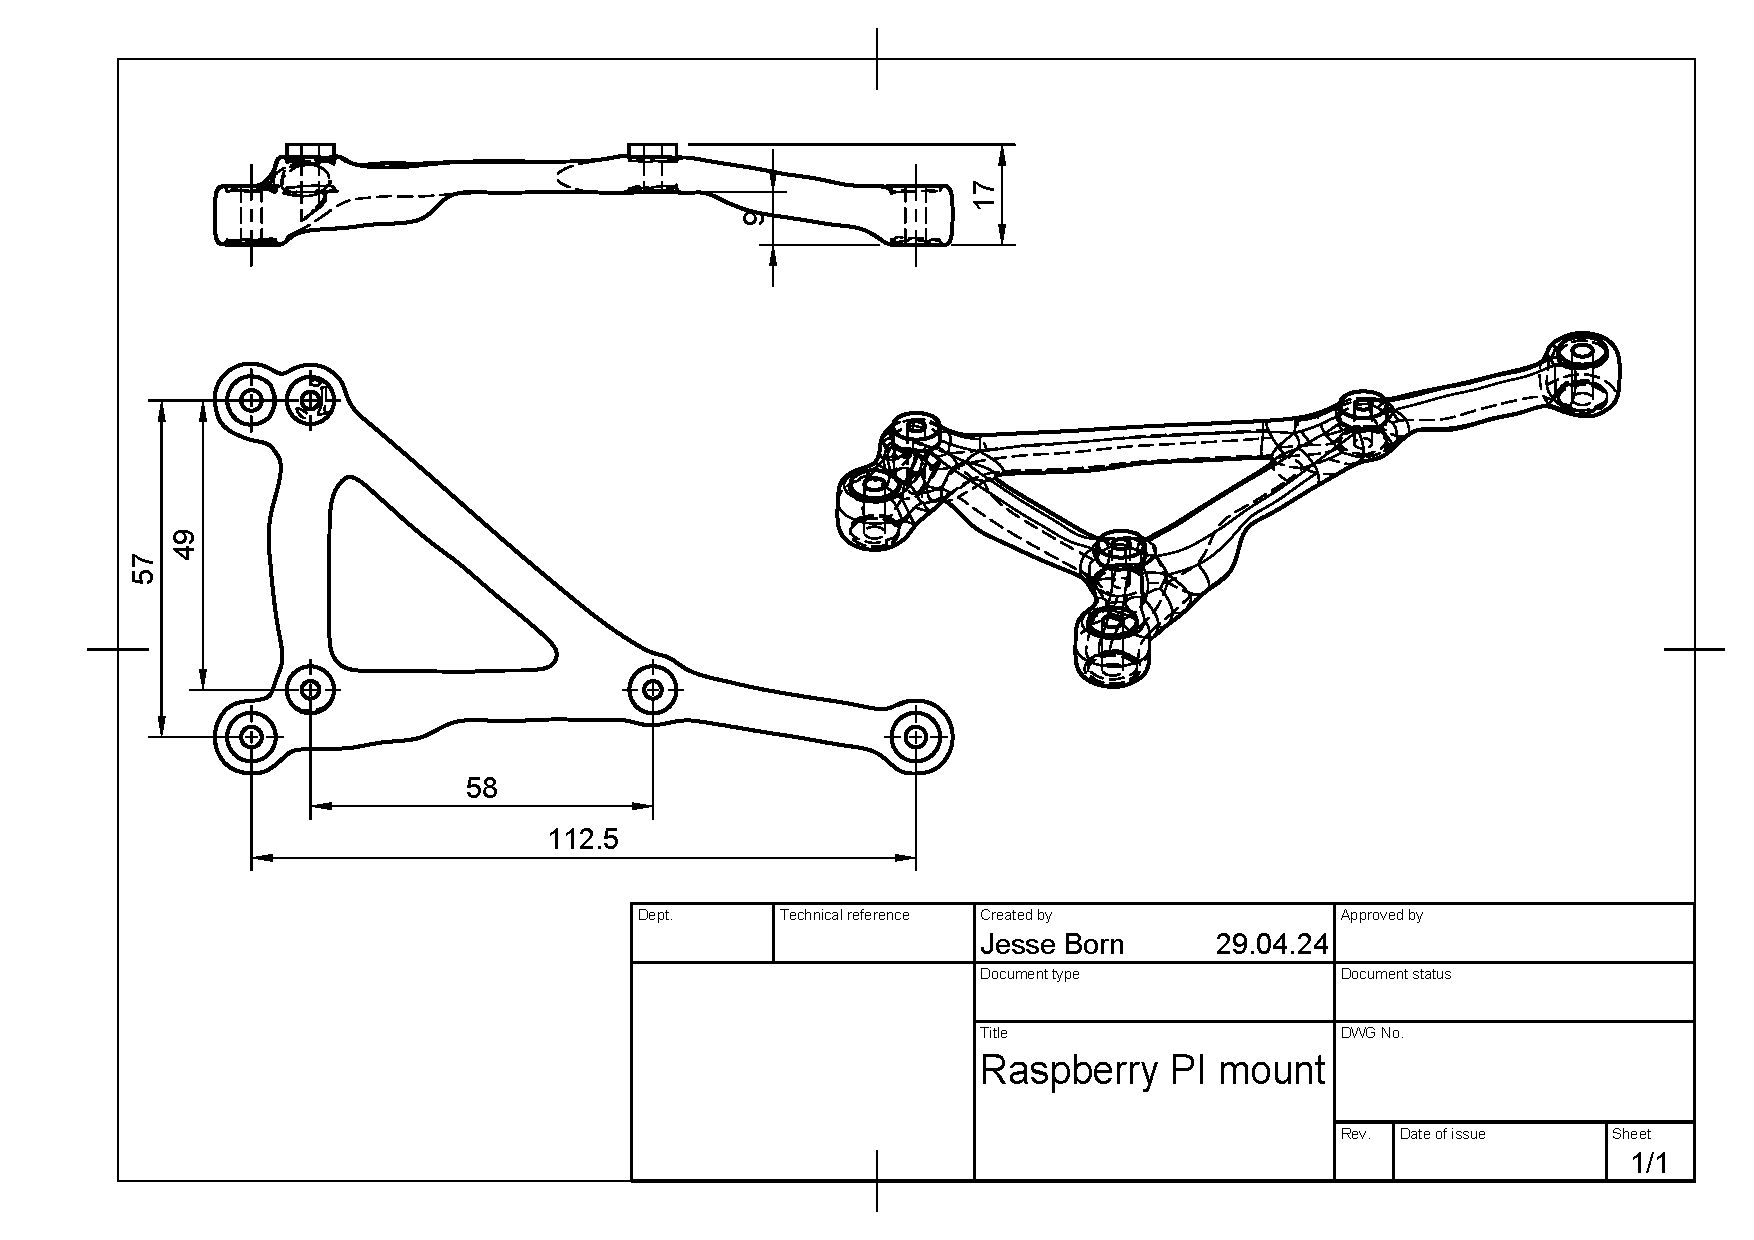
\includepdf[landscape=true]{plans/raspberrypiholder.pdf}
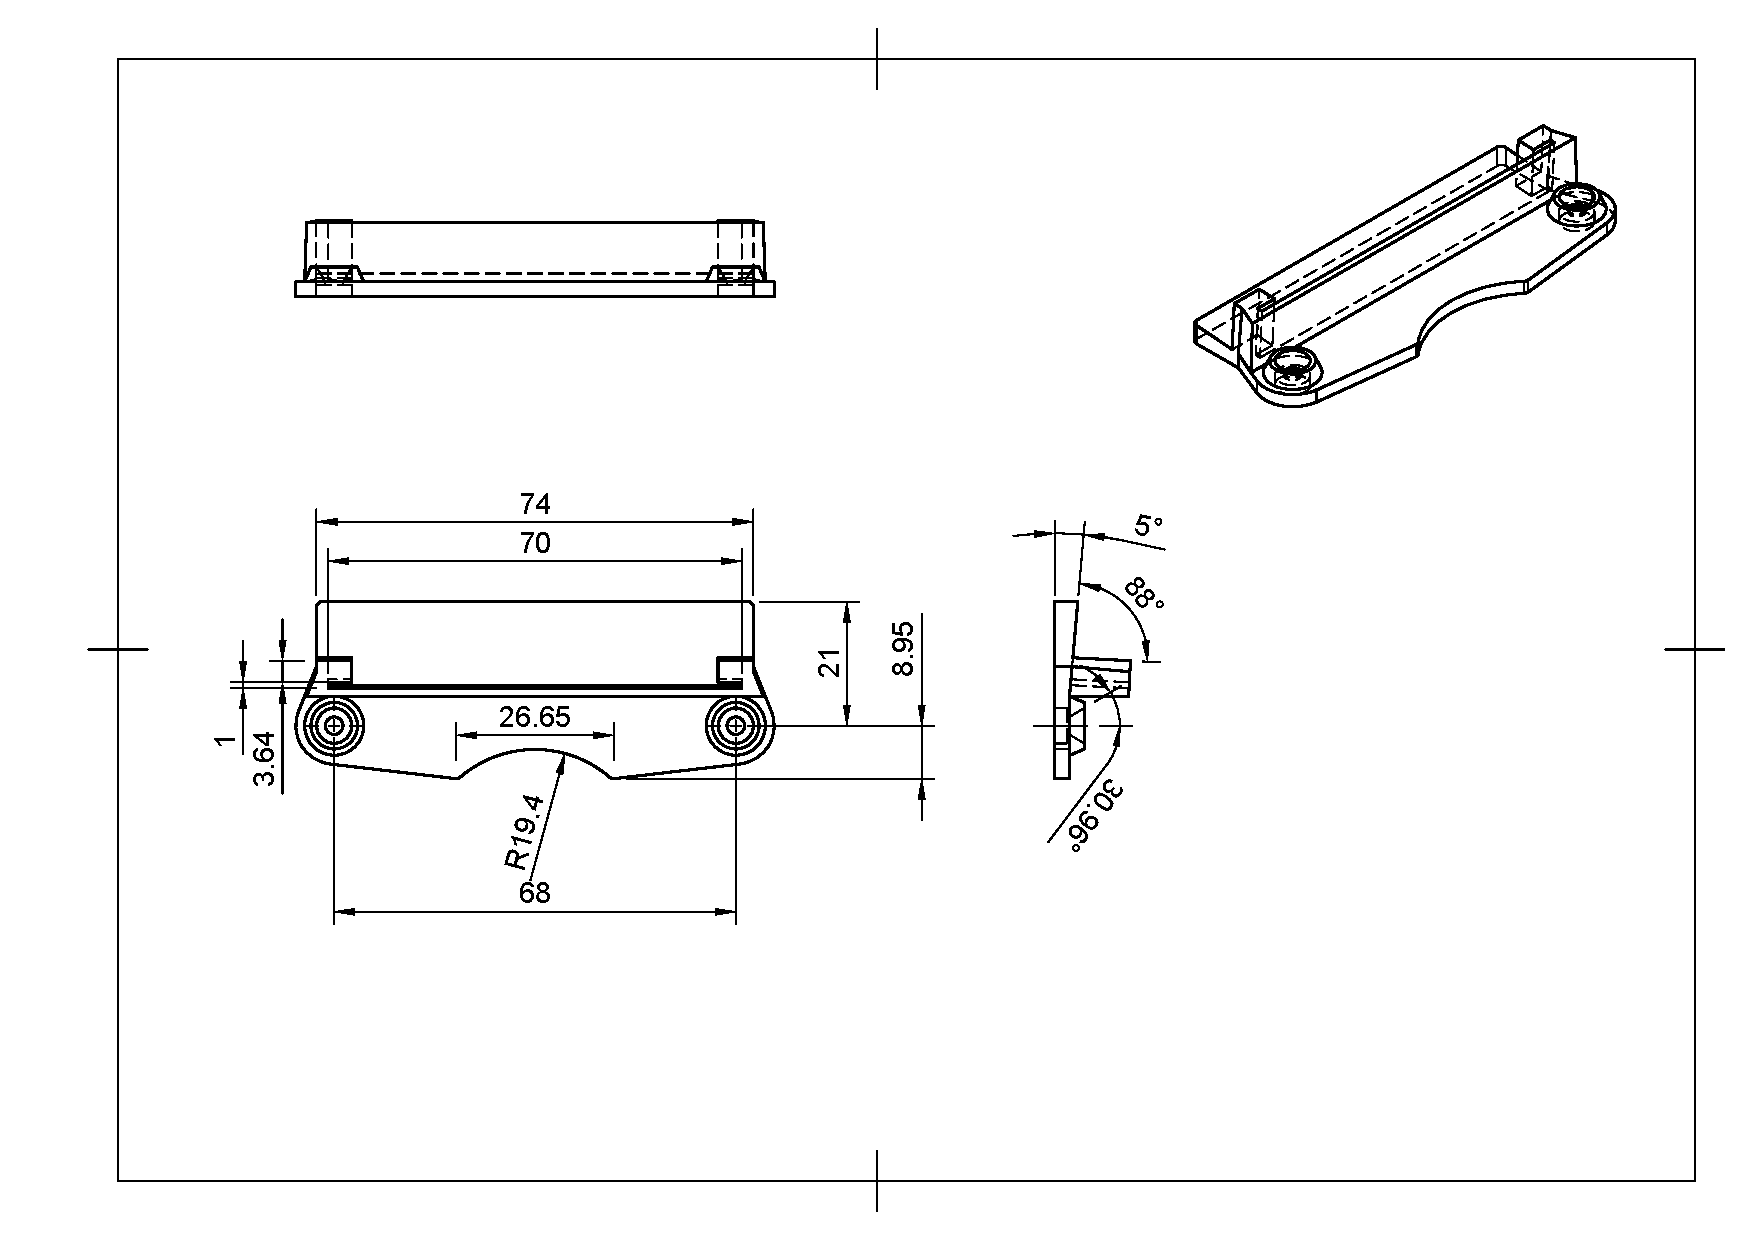
\includepdf[landscape=true]{plans/cameraholder.pdf}
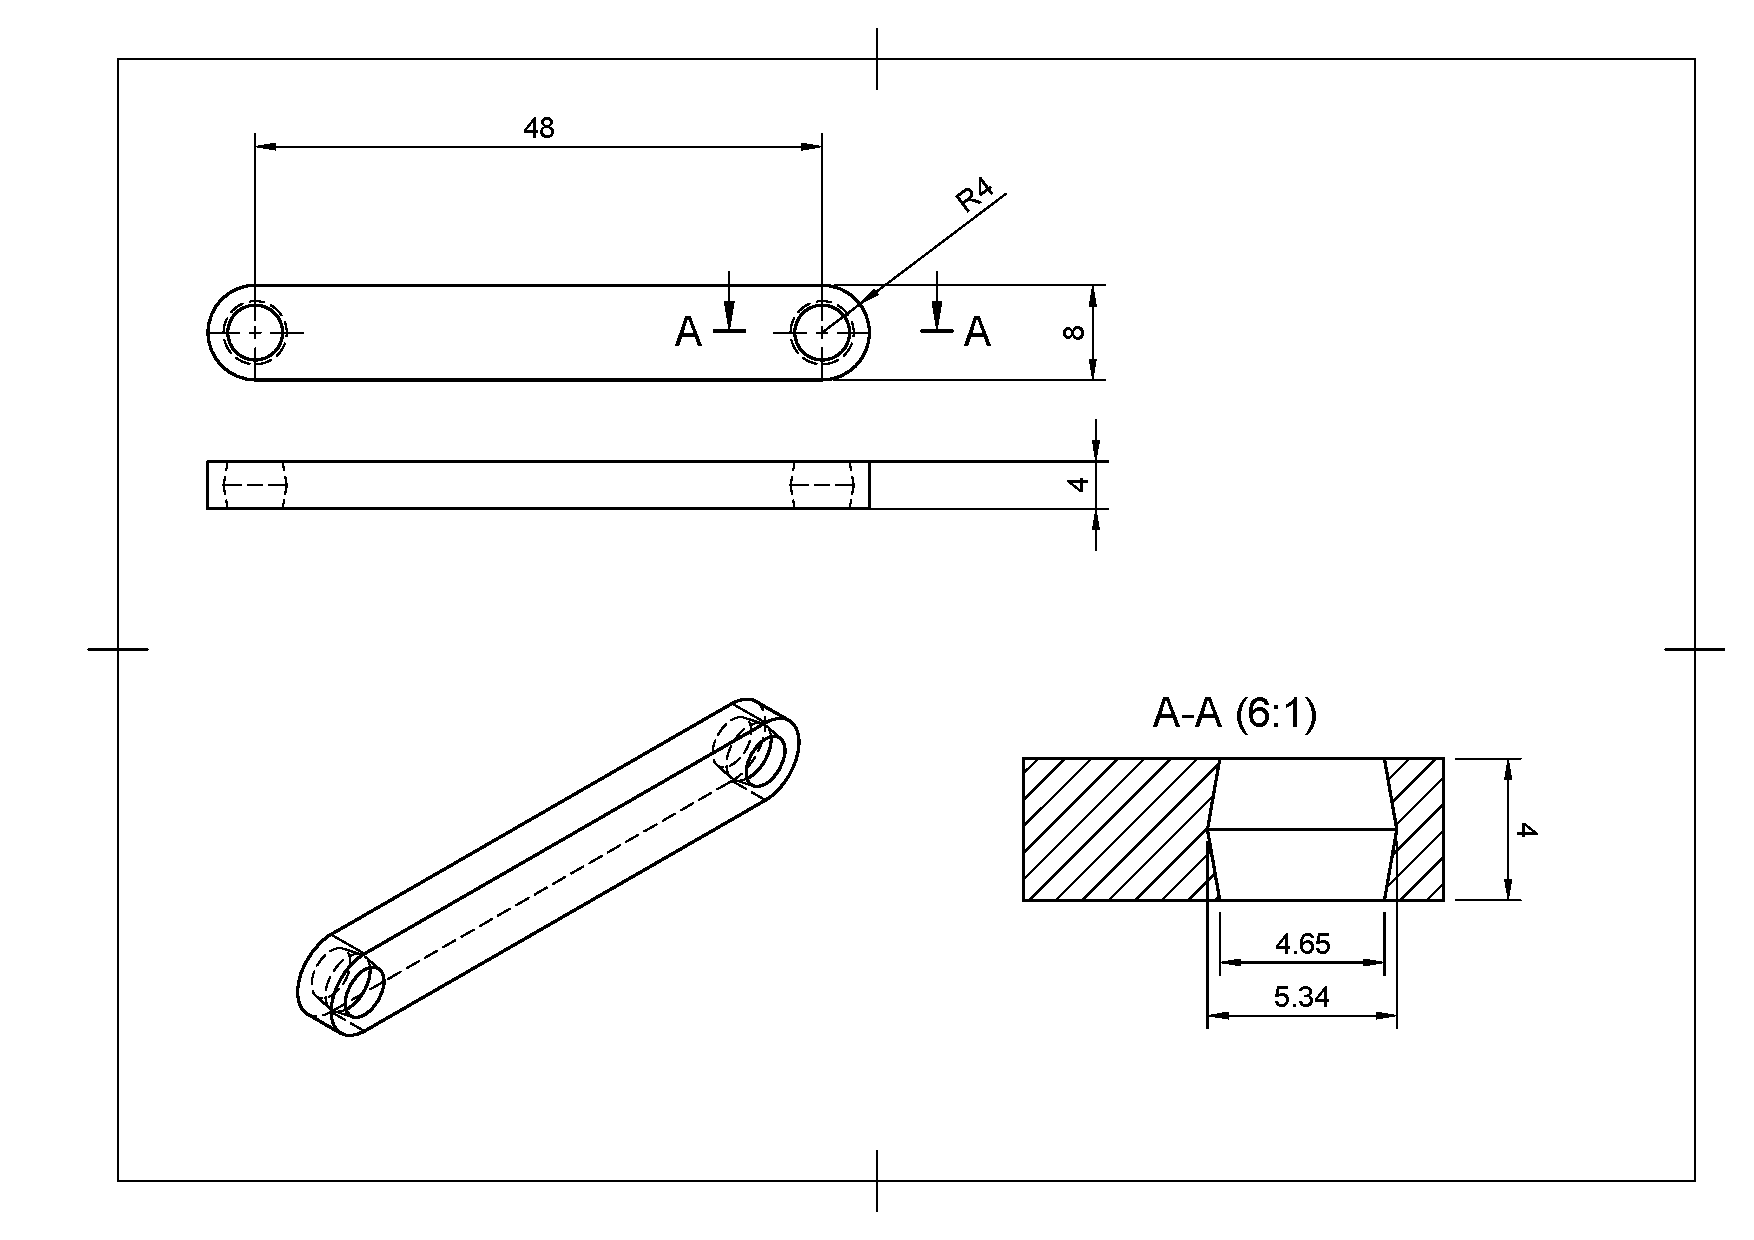
\includepdf[landscape=true]{plans/suspension.pdf}

% 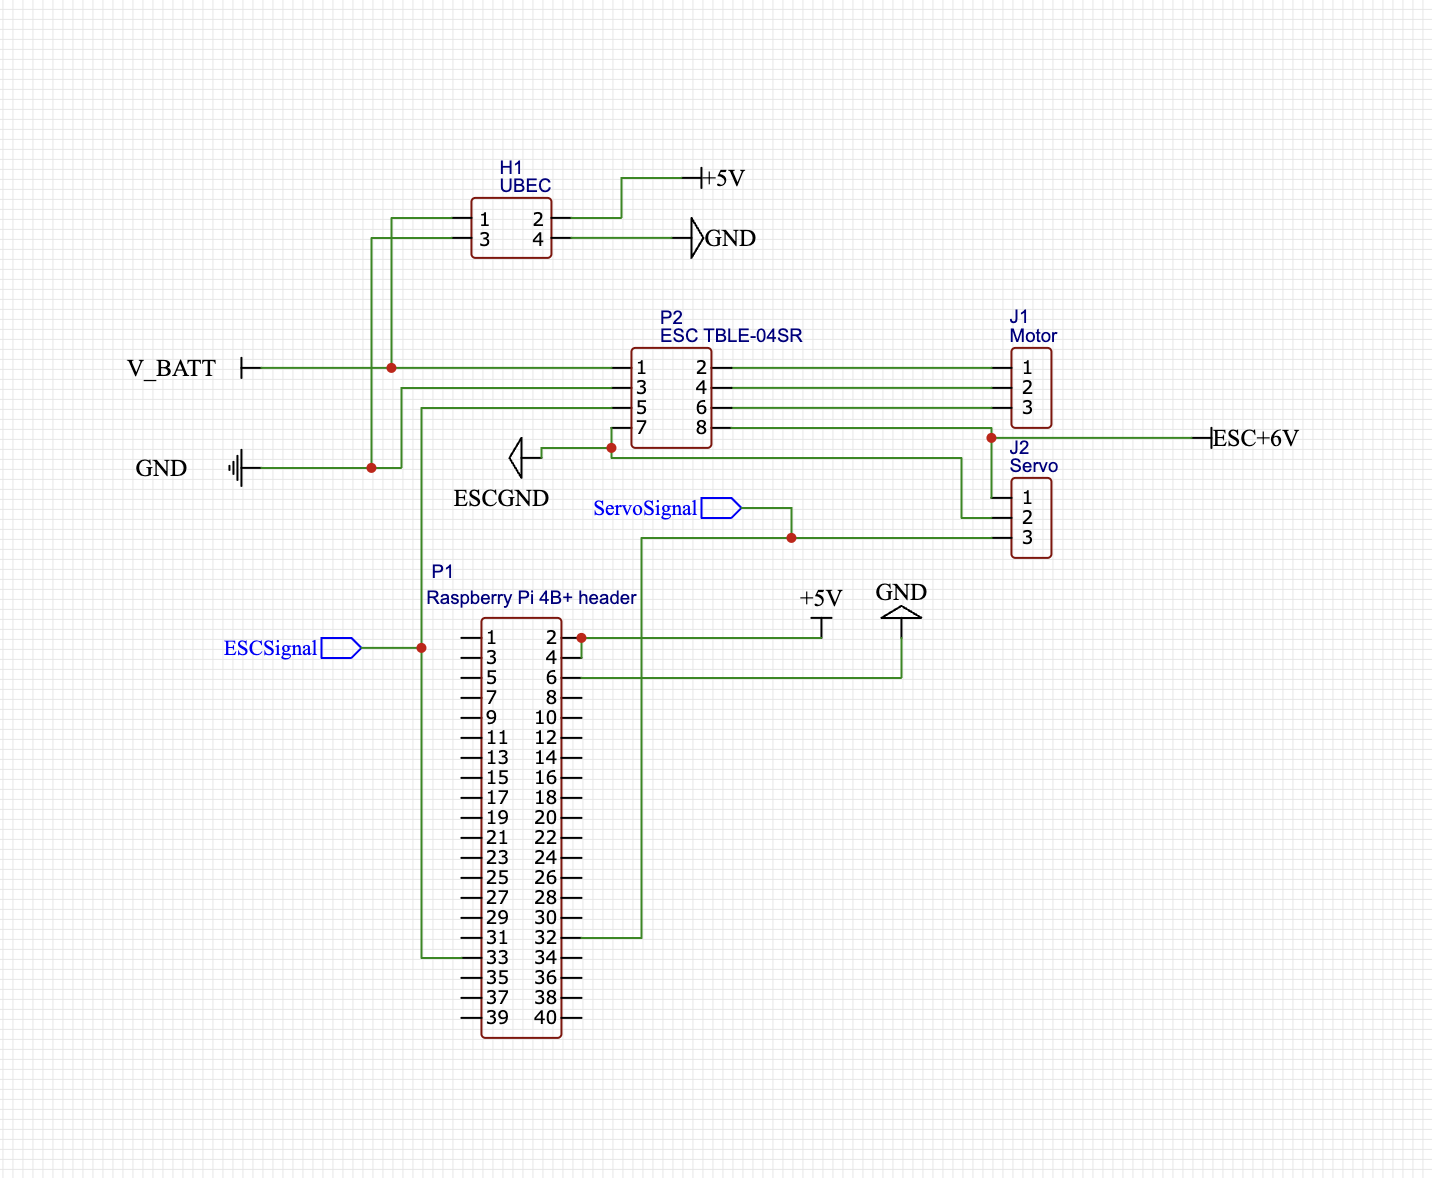
\includegraphics[width=16cm]{circuit.png}

\end{document}
